\documentclass[11pt]{jsarticle}

\usepackage[top=30mm, bottom=36mm, left=28mm, right=28mm]{geometry}
\usepackage[dvipdfmx]{graphicx}

\usepackage{mytitle}

\title{2. ストリーム処理の基本}
\author{201720690 小松 弘人}
\date{2017/06/12}

\makeatletter
\def\mojiparline#1{
    \newcounter{mpl}
    \setcounter{mpl}{#1}
    \@tempdima=\linewidth
    \advance\@tempdima by-\value{mpl}zw
    \addtocounter{mpl}{-1}
    \divide\@tempdima by \value{mpl}
    \advance\kanjiskip by\@tempdima
    \advance\parindent by\@tempdima
}
\makeatother
\def\linesparpage#1{
    \baselineskip=\textheight
    \divide\baselineskip by #1
}

\begin{document}
\maketitle
\subsection*{ストリーム処理}
FPGAで画像処理を行う場合、フレームバッファを用意して画像全体を格納する方法と、
画像データをラスタスキャン順に送信し、順次処理をしていく方法がある。
後者を、ストリーム処理という。
ここでは、図\ref{img:raster}のように画像データをFPGAに送り、
カーネルサイズが$3\!\times\!3$の線形フィルタを適用する構成を考える。

\begin{figure}[ht]
	\centering
	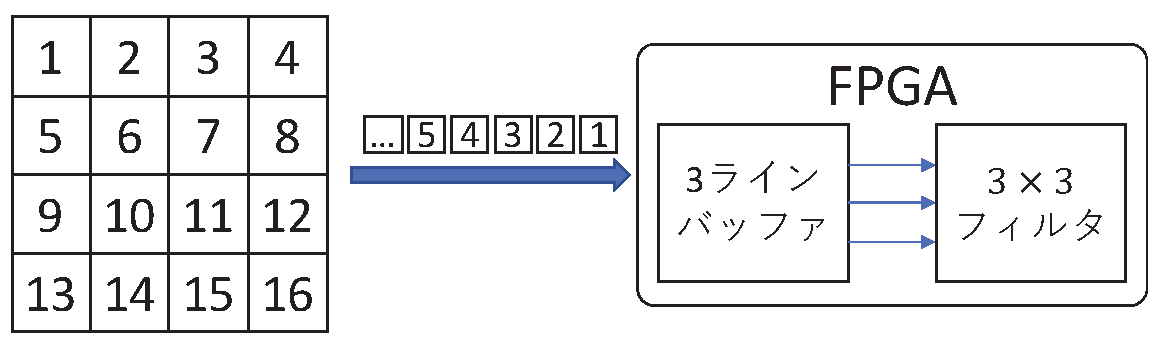
\includegraphics[width=0.7\linewidth]{img/raster.pdf}
	\caption{システム構成}
	\label{img:raster}
\end{figure}

\vspace{-0.5cm}

$3\!\times\!3$のフィルタを計算するためには、
注目画素とその8近傍のデータが必要となる。
このデータを用意するために、3ラインバッファが用いられる。
3ラインバッファは、画像の3行分のデータを格納し、
後段の回路に提供するための回路である (図\ref{img:3linebuf})。
3ラインバッファは、FIFO IP Coreを3つ連結して作成できる (図\ref{img:3lb_fifo})。

\begin{figure}[ht]
	\centering
	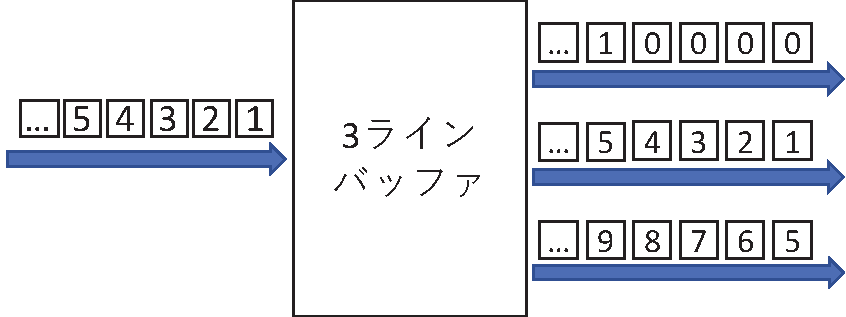
\includegraphics[width=0.5\linewidth]{img/3lb.pdf}
	\caption{3ラインバッファの動作}
	\label{img:3linebuf}
\end{figure}

\vspace{-0.5cm}

\begin{figure}[ht]
	\centering
	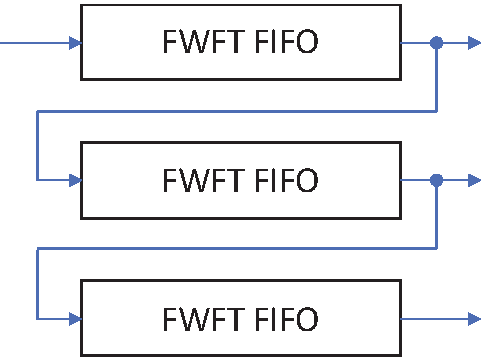
\includegraphics[width=0.3\linewidth]{img/3lb_fifo.pdf}
	\caption{3ラインバッファの概念図}
	\label{img:3lb_fifo}
\end{figure}

$3\!\times\!3$フィルタモジュールでは、
3ラインバッファの出力をレジスタに格納し、
$3\!\times\!3$のデータを用意し、計算を行う。
このとき、計算をパイプライン化し、並列処理することで
スループットを向上させることを目指す。
これにより、画像フィルタを高速に計算できる。

\end{document}
